
%%%%%%%%%
%% Results and Discussion
\section{Results and Discussion}
After the four measurement runs completed on Shout, we perform an analysis with the SPLAT! tool using the same frequencies, 
radio locations and following the same method discussed in Section~\ref{sec:method}.
We convert our acquired data into plots through the use of our python script. 
Each dot on the plot is a pairwise connection between the transmitter
and receiver at the given frequency. Due to the multitude of dots we refrain from naming each dot as it overwhelms the plot. Due to the unknown reference for either Shout or SPLAT! we are unable to directly compare the two.
However, we will compare the two using the path loss exponent which happens to be the slope of the linear regression line of transmission power versus distance plot. 
Following the path loss exponent analysis we will do a brief terrain analysis of the results we obtained. 

\subsection{Path Loss Exponent}
Due to the POWDER platforms uncalibrated radios there is not a single reference point for the Shout data. This is the reason 
why all of our plots for each run define the Y-axis as the received power in dBm with an unknown reference. Notice that SPLAT!'s
data is represented by the red color while Shout's data is represented by the blue color. Table~\ref{tab1} summarizes the path 
loss exponents for each run.

Run 1 (Fig.~\ref{3561}), was conducted on the 3561 MHz frequency in early October 2020 at around 11AM. This run followed
the typical round-robin fashion, where each circle on the plot represents a pairwise connection between the transmitter and receiver. 
The slope for Shout in run 1 was $-0.00862$, this tells us that the power decays proportionally to $d^{-0.00862}$ where $d$ is the 
path length. Similarly, we determined the measurements fit of SPLAT!. The path loss exponent is $-0.0154$ that is the power decays 
proportionally to $d^{-0.0154}$. We can see SPLAT!'s path loss exponent has a steeper slope. That is for the 3561 
\begin{figure}[htbp]
\centerline{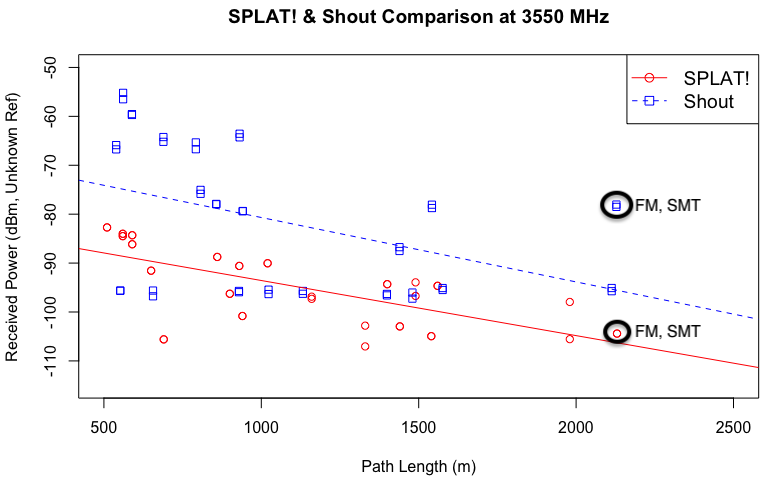
\includegraphics[width=0.9\columnwidth]{figs/3550.png}}
\vspace{-3mm}
\caption{Run 3. Used 3550 MHz frequency.}
\label{3550}
\vspace{-3mm}
\end{figure}
\begin{table}[htbp]
\caption{Run 1, best path loss for Shout and SPLAT!}
\begin{center}
\begin{tabular}{|c|c|c|}
\hline
\textbf{Data Set} & \textbf{\textit{Nodes}}& \textbf{\textit{Received Power (dBm)}} \\
\hline
Shout& MEB, Browning& $-52$ \\
SPLAT!& MEB, Browning& $-83$ \\
\hline
\end{tabular}
\vspace{-3mm}
\label{tab2}
\end{center}
\end{table}
MHz frequency, SPLAT! has over-predicted the path loss when compared to Shout's ground truth measurements. 

We now conduct a similar procedure for the remaining runs. Run 2 (Fig.~\ref{2620}) was conducted in early November 2020 at
around 9AM and used the largest amount of nodes within our experiments. Shout's path loss exponent was $-0.0114$ with a power 
decay proportional to $d^{-0.0114}$. While SPLAT!'s path loss exponent was $-0.0186$ with a power decay proportional to 
$d^{-0.0186}$. These are fairly close but once again SPLAT! is over-predicting the POWDER platform's radio path loss at the 2620 
MHz frequency. 

Run 3 (Fig.~\ref{3550}) and run 4 (Fig.~\ref{3690}) were conducted in late November 2020. Specifically, run 3 was 
conducted at around 2AM while run 4 occurred around 6AM. For run 3, Shout's path loss exponent is $-0.0132$ while SPLAT!'s 
is $-0.0113$. Run 3 offers the closest in comparing the path loss exponent values for the data collected. However, this time SPLAT! 
is under-predicting the POWDER platforms path loss for the 3550 MHz frequency. Similarly, in run 4 we see SPLAT! under-predicting
the path loss on the 3690 MHz frequency. In run 4 we see that Shout's path loss exponent is $-0.0163$, while SPLAT!'s path loss 
exponent is $-0.0103$. 

\subsection{Terrain Analysis}
The purpose of this section is to bring SPLAT! to real life and compare the model to physical locations. We utilize Google 
Maps to take a closer view of the environment in run 1. Notice that in Fig.~\ref{3561}, we label the best and worst path loss 
nodes for each data set. We will focus on the two nodes with the best path loss, and the two nodes with the worst path loss and 
compare Shout and SPLAT! when differences arise. 

\subsubsection{Best Path Loss}
We first look at the two nodes in run 1 with the best path loss. Table~\ref{tab2} lists the best path loss nodes for both Shout and 
SPLAT!, at the 3561~MHz frequency. We can see that for both data sets, MEB and Browning hold the best propagation values. 
Fig.~\ref{mebBrown} shows the Google Maps
\begin{figure}[htbp]
\centerline{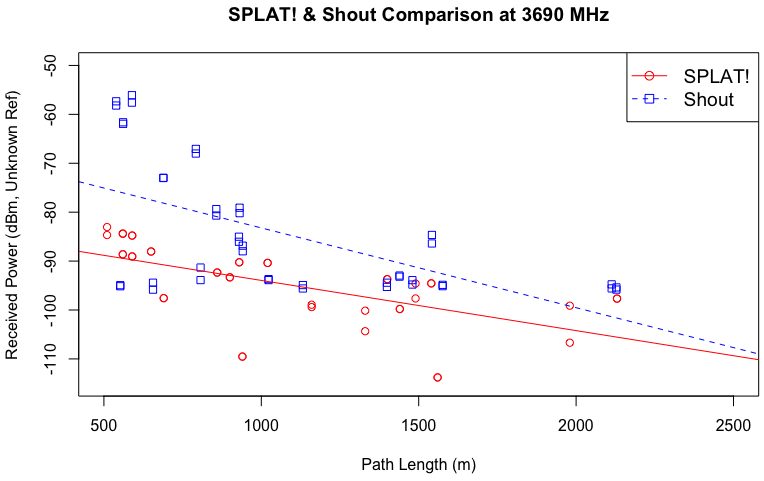
\includegraphics[width=0.9\columnwidth]{figs/3690.png}}
\vspace{-3mm}
\caption{Run 4. Used 3690 MHz frequency.}
\label{3690}
\vspace{-3mm}
\end{figure}
\begin{table}[htbp]
\caption{Run 1, worst path loss for Shout and SPLAT!}
\begin{center}
\begin{tabular}{|c|c|c|}
\hline
\textbf{Data Set} & \textbf{\textit{Nodes}}& \textbf{\textit{Received Power (dBm)}} \\
\hline
Shout& MEB, SMT& $-87$ \\
SPLAT!& MEB, Sagepoint& $-115$ \\
\hline
\end{tabular}
\label{tab3}
\vspace{-3mm}
\end{center}
\end{table}
image of the two nodes. Both nodes are rooftop base stations with LOS. We believe that these two nodes received the
best propagation simply due to the distance between them and the fact that there is 
nothing directly blocking them.  

\subsubsection{Worst Path Loss}
We now look at the two worst nodes with regards to propagation loss. Table~\ref{tab3} lists the worst path loss nodes for both 
Shout and SPLAT! at the 3561~MHz frequency. For SPLAT! these two nodes are MEB and Sagepoint. We note that Sagepoint 
is the only fixed endpoint node for run 1 and is 1.5~meters above the ground, while MEB is a rooftop base station. From 
Fig.~\ref{worst} we notice that the environment between MEB and Sagepoint is NLOS. In fact, three sports fields, the student
life center, a busy road, and multiple housing units lie in-between these two nodes. Furthermore, since Sagepoint is a 
fixed endpoint node it is placed behind a wall that is not facing the MEB. 

However, Shout thinks differently. It believes that the two worst nodes are MEB, and South Medical Tower (SMT). The environment
between these two include the Biotechnology Building, a busy road, parking structures, and the College of Pharmacy.
However, both MEB and SMT are rooftop base stations with MEB being the shorter one. 

\subsection{Discussion}
We now offer a few insights as to why we got the results we did. We can see how early hours affected Shout's data in run 3. 
In Fig.~\ref{3550} where we can see that at a striking distance of about 2128 meters we appear to be getting $-78$ dBm 
in received power compared to SPLAT!'s $-104$ dBm, for the Friendship Manor and SMT nodes. Again we can't compare 
point-to-point due to unknown reference, but this appears to be an outlier
when compared to the rest of Shout's data where 
about half the points are underneath $-78$ dBm given their respective smaller path length.

\begin{figure}[htbp]
\centerline{\includegraphics[width=0.9\columnwidth]{figs/mebBrown.png}}
\caption{MEB left and Browning right.}
\label{mebBrown}
\vspace{-3mm}
\end{figure}

\begin{figure}[htbp]
\centerline{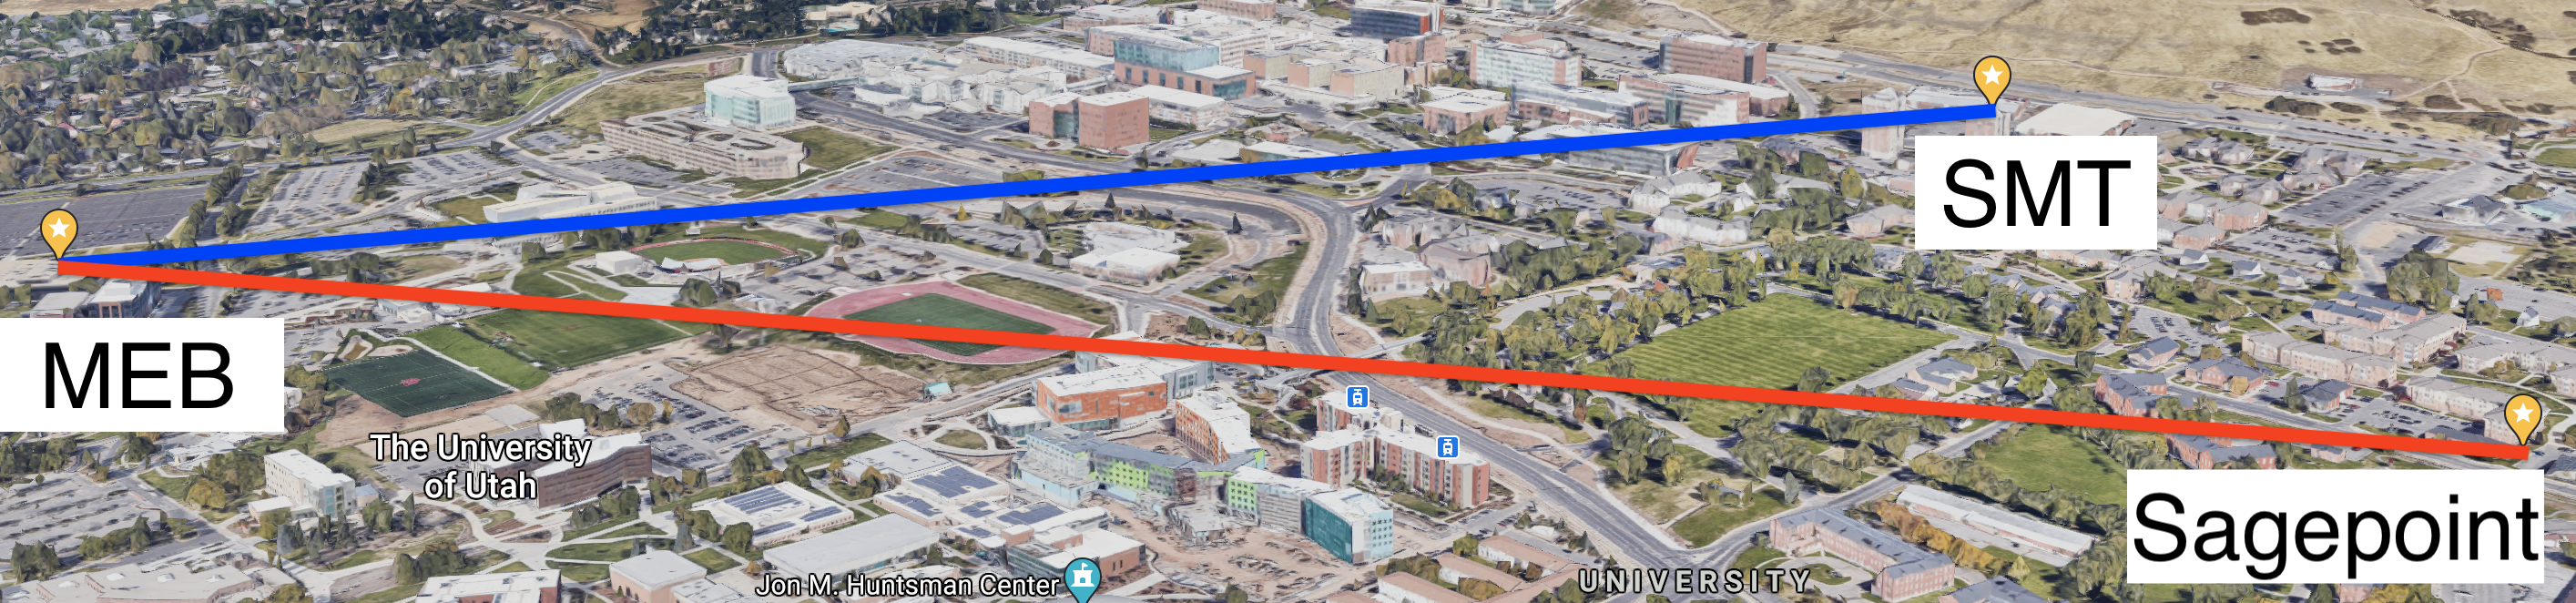
\includegraphics[width=0.9\columnwidth]{figs/worst.png}}
\caption{SPLAT! (Red): MEB to Sagepoint; Shout (Blue): MEB to SMT.}
\label{worst}
\vspace{-3mm}
\end{figure}

As expected for all cases in every run we saw power levels with exponentially decreasing magnitude as a function of 
distance. Meaning that in all cases we saw propagation loss increase with distance. As discussed in the background section, 
there exists multiple path loss models that can be used depending on the parameters available to us. For example, SPLAT! 
follows the Longley-Rice path loss model, and this model might not be sophisticated
enough to accomodate the topology found in our experiment.

Note that our goal with this work is not to evaluate the accuracy of the SPLAT! tool
per se, but rather to illustrate the utility of the POWDER platform to conduct research 
of this nature. Specifically, the ability to perform longitudinal studies on POWDER, spanning different weather conditions and seasons, coupled with the flexibility
and rich diversity of the platform, suggests the usefulness of POWDER for this type of
research.   
